\documentclass[conference]{IEEEtran}
\IEEEoverridecommandlockouts
% The preceding line is only needed to identify funding in the first footnote. If that is unneeded, please comment it out.
%Template version as of 6/27/2024

\usepackage{cite}
\usepackage{amsmath,amssymb,amsfonts}
\usepackage{algorithmic}
\usepackage{graphicx}
\usepackage{textcomp}
\usepackage{xcolor}
\usepackage{url}
\def\BibTeX{{\rm B\kern-.05em{\sc i\kern-.025em b}\kern-.08em
    T\kern-.1667em\lower.7ex\hbox{E}\kern-.125emX}}
\usepackage{float}
\begin{document}

\title{Customer Segmentation for an Online Store using K-Means Clustering\\


}

\author{\IEEEauthorblockN{1\textsuperscript{st} Md Limon Mia}
\IEEEauthorblockA{\textit{dept. Computer Science and Engineering} \\
\textit{Dhaka International University}\\
Dhaka, Bangladesh \\
mdhlimonmia@gmail.com}
\and
\IEEEauthorblockN{2\textsuperscript{nd} Ananna Rani Dash}
\IEEEauthorblockA{\textit{dept. Computer Science and Engineering} \\
\textit{Dhaka International University}\\
Dhaka, Bnagladesh \\
dristy202008@gmail.com}
}

\maketitle

\begin{abstract}
Customer segmentation is a powerful strategy used in e-commerce to enhance personalized marketing and increase customer retention. This research focuses on implementing K-Means clustering to identify distinct customer groups based on their behavioral attributes such as annual income and spending patterns. Using a real-world e-commerce dataset, data preprocessing and scaling techniques were applied to prepare the data for clustering. The Elbow Method was employed to determine the optimal number of clusters. The results provided clear segmentation of customers into groups, helping businesses target each group more effectively. This paper demonstrates how machine learning techniques can be applied to customer data to produce actionable business insights.
\end{abstract}

\begin{IEEEkeywords}
Customer segmentation, K-Means, Machine Learning, E-Commerce, Clustering, Scikit-learn
\end{IEEEkeywords}

\section{Introduction}
The rapid growth of e-commerce has significantly increased the volume of customer data collected by online retailers. Understanding and leveraging this data has become essential for businesses to remain competitive. One effective approach is customer segmentation, which involves grouping customers based on shared characteristics or behaviors. This process allows businesses to tailor marketing efforts, personalize user experiences, and improve customer satisfaction.

Customer segmentation can be achieved using various statistical and machine learning techniques. Among them, K-Means clustering is widely adopted due to its simplicity, efficiency, and interpretability.

\section{Literature Review}
Several studies have highlighted the importance of customer segmentation in improving marketing performance and customer satisfaction. Traditional segmentation approaches rely on demographic data or manual classification. However, with the advancement of machine learning, unsupervised clustering algorithms such as K-Means, DBSCAN, and hierarchical clustering have gained popularity.

K-Means is particularly effective in scenarios where the number of segments is known or can be estimated. The algorithm partitions customers into $k$ groups by minimizing intra-cluster variance. Research has shown that this method yields meaningful insights into customer behavior.

\section{Methodology}
This study uses the K-Means clustering algorithm to identify customer segments in an online store. The analysis was conducted using Python libraries such as \texttt{pandas}, \texttt{scikit-learn}, and \texttt{matplotlib}. The methodology followed these steps:

\begin{enumerate}
    \item \textbf{Data Collection}: A public e-commerce dataset containing features such as `CustomerID`, `Age`, `Annual Income (k\$)`, and `Spending Score (1–100)` was used.
    \item \textbf{Dataset Description}: The dataset used in this study contains anonymized records of customers from an e-commerce platform. Key attributes include:
        \begin{itemize}
          \item Customer ID
          \item Gender
          \item Age
          \item Annual Income
          \item Spending Score
        \end{itemize}
    \item \textbf{Data Preprocessing}:The dataset was cleaned by removing missing values and irrelevant columns. Actually this dataset already perfect but I also checked. Here preprocessing steps included:
        \begin{itemize}
          \item Handling missing values
          \item Selecting relevant features: \textbf{Annual Income} and \textbf{Spending Score}
          \item  Standardizing features using \textbf{StandardScaler} from \textbf{scikit-learn}
        \end{itemize}
    \item \textbf{Feature Selection}: Only numerical attributes (`Annual Income`, `Spending Score`) were selected for clustering.
    \item \textbf{Feature Scaling}: To ensure all features contribute equally to the distance calculations in \textbf{K-Means}, feature scaling was applied:
\begin{verbatim}
from sklearn.preprocessing import
 StandardScaler
scaler = StandardScaler()
x_scaled = scaler.fit_transform(x)
\end{verbatim}
    \item \textbf{Determining the Number of Clusters}: The Elbow Method was used to determine the best number of clusters (k\$):
\begin{verbatim}
# Elbo Method to find optimal k
arr = []
for k in range(1, 11):
 kmeans = KMeans(n_clusters=k,
  init='k-means++', random_state=42)
  
 kmeans.fit(x_scaled)
 arr.append(kmeans.inertia_)
 plt.figure(figsize=(10, 5))
 plt.plot(range(1, 11), arr,
  marker='o',color='b', 
  linestyle='-', markersize=6)
plt.title('Elbow Method to Determine 
  Optimal k')
plt.xlabel('Number of Clusters')
plt.ylabel('Inertia')
plt.grid(True)
plt.show()
\end{verbatim}
        
        \begin{figure}[h]
            \centering
            \includegraphics[width=0.45\textwidth]{elbow_plot.png}
            \caption{Elbow Method for optimal number of clusters}
            \label{fig:elbow}
        \end{figure}
    \item \textbf{Applying K-Means Clustering}: K-Means clustering was applied to the data. Based on the Elbow Method, 5 clusters were selected:
\begin{verbatim}
optimal_k = 5
kmeans = KMeans(n_clusters= optimal_k,
 init = 'k-means++', random_state= 42)
y = kmeans.fit_predict(x_scaled)
\end{verbatim}

    \item \textbf{Visualization}: Cluster results were visualized using a 2D scatter plot.
\begin{verbatim}
cluster_labels = {
0: 'Low Income, Low Spending',
1: 'High Income, High Spending',
2: 'Moderate Income, High Spending',
3: 'High Income, Low Spending',
4: 'Moderate Income, Low Spending'
}

plt.figure(figsize=(10, 6))
for lbl, name in cluster_labels
   .items():
 plt.scatter(x_scaled[y == lbl, 0], 
 x_scaled[y == lbl, 1],  label=name,
 s = 40)
plt.xlabel('Annual Income (k$)')
plt.ylabel('Spending Score (1-100)')
plt.title('Customer Segmentation
 using KMeans')
plt.legend()
plt.grid(True)
plt.show()
\end{verbatim}
\end{enumerate}

\section{Results}
After applying the Elbow Method, the optimal number of clusters was found to be 5. K-Means was then applied, and customers were grouped based on their income and spending scores.
\begin{figure}[h]
    \centering
    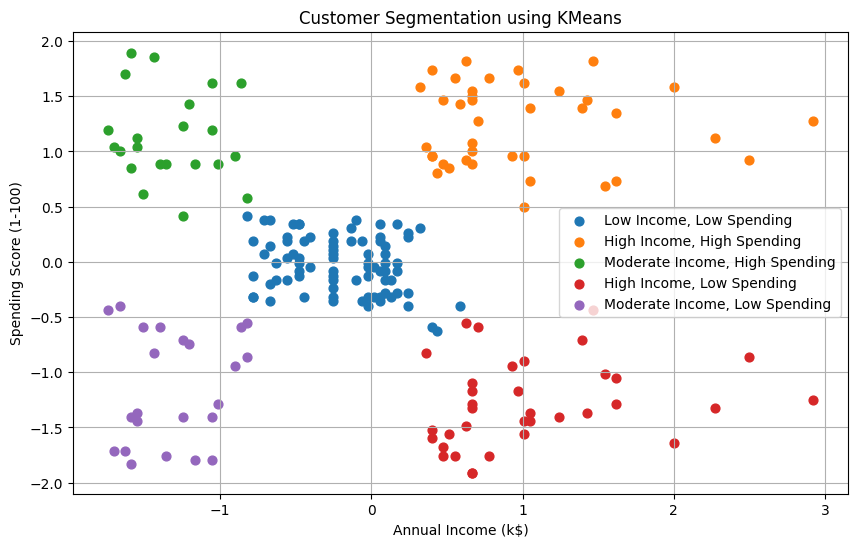
\includegraphics[width=0.45\textwidth]{customer_segment.png}
    \caption{Customer segmentation using K-Means}
    \label{fig:clusters}
\end{figure}

\begin{table}[H]
\centering
\caption{Summary of Customer Segments}
\begin{tabular}{|l|c|c|}
\hline
\textbf{Segment} & \textbf{Avg. Income (k\$)} & \textbf{Avg. Score} \\
\hline
Low Income, Low Spending       & 55.30 & 49.25 \\
High Income, High Spending     & 86.54 & 82.13 \\
Moderate Income, High Spending & 25.73 & 79.36 \\
High Income, Low Spending      & 88.20 & 17.11 \\
Moderate Income, Low Spending     & 26.30 & 20.91 \\
\hline
\end{tabular}
\end{table}


Each cluster represented a group of customers with similar purchasing behavior. For instance, one group had high income but low spending, indicating potential targets for special promotions.

\section{Discussion}
Segmentation revealed meaningful patterns in customer behavior. Businesses can now apply tailored strategies for each segment, such as:

\begin{itemize}
    \item Offering discounts to low-spending high-income groups
    \item Rewarding loyal high-spending customers
    \item Creating budget-friendly deals for low-income segments
\end{itemize}

\section{Conclusion}
This research demonstrates how customer segmentation using K-Means clustering can uncover valuable insights from e-commerce customer data. The clustering revealed meaningful patterns in customer behavior that can directly inform marketing strategies and resource allocation. By identifying groups such as high spenders and low-engagement customers, businesses can tailor their approaches to different customer types more effectively.

\section*{Acknowledgment}
The author would like to thank the open-source community and dataset providers for making the data accessible.
% Reference
\begin{thebibliography}{1}

\bibitem{sklearn}
 Jain, A. K. (2010). Data clustering: 50 years beyond K-means. *Pattern Recognition Letters.

\bibitem{kaggle}
Vijay Choudhary, “Customer Segmentation Dataset,” Kaggle. [Online]. Available: \url{https://www.kaggle.com/datasets/vjchoudhary7/customer-segmentation-tutorial-in-python}

\bibitem{marketing}
Kotler, P., and Keller, K.L., “Marketing Management,” 15th ed., Pearson Education, 2016.
\bibitem{marketing}
https://www.analyticsvidhya.com/blog/2019/08/comprehensive-guide-k-means-clustering/

\end{thebibliography}

\end{document}
